% !TEX TS-program = XeLaTeX
% !TEX encoding = UTF-8 Unicode

\chapter{系统设计}

\label{系统设计}

\defaultfont

\section{系统架构设计}

如图\ref{system-frame-deployment}所示,本系统采用的时前后端分离架构,系统前端使用vue,Element Plus UI,axios,vuex,vue-router,系统后端使用了Spring Boot,同时配置Tomcat,Spring Security,Spring Data JPA,系统的持久化选择Hibernate和MySQL。

前后端分离架构优势:

(1) 系统的可伸缩性

由于将代码分成前端和后端两部分,可以不用考虑对方进行独立优化,只要保证数据接口不改变,那么双方的交互就不会出现问题。

(2) 减少资源传递

在以往的非前后端分离项目中,服务器要做的工作有解析请求,从数据库中检索相关数据并处理数据,然后结合HTML模板并将其发送给浏览器。而在前后端分离的系统中,服务器并不需要处理HTML,之需要将处理好的数据作为response(一般是JSON对象)返还给前端,而前端根据数据进行展示,这个过程减少了服务器的任务,因此降低了服务器的压力,并且用户体验更好,因为整个页面不会随着每个请求而更新。

(3) 更容易升级

升级架构是一件痛苦的事情。前后端分离可以更好地进行升级和调试,通过查看接口返回数据的正确与否就可以判断是前端的问题还是后端的问题,这在系统升级的过程中可以加速问题的排查。

(4) 更容易切换框架

现如今技术的的变化很快,不仅现在使用的框架更新频率很高,并且新的更好的框架也层出不穷。在使用前后端分离架构的情况下,前后端并不关心对方使用的是什么框架,只需要规定好接口并且保证在切换框架的过程同接口不会改变。比如前端从Vue转变为Angular,这个变化后端并不会有感知。

(5) 更快地部署

由于前端开发人员和后端开发人员并不需要太多地相互依赖(只有在定义接口的时候需要双方协商),所以前后端可以独立进行测试和部署而无需等待对方任务的完成。

(6) 整合的API

当前端需要多平台部署时,例如Web端,移动端,在开发应用的过程中,不需要为各自的编写不同的后台,两者可以使用相同的后台,即使用相同的API,这无疑减小了不必要的、重复的代码编写。而且在使用相同的API的情况下可以保证各个平台的数据的一致性,以及后台升级时,各个平台同时获得更新。

(7) 模块化

如果您的前端与后端分离,那么在一个模块上工作而不影响另一个模块就变得更容易了。模块化还使两个团队或两个人同时在前端和后端工作变得更容易,而不必担心覆盖或搞乱其他人的工作。他们也可以用不同的节奏工作。

\begin{figure}[htbp]
    \centering
    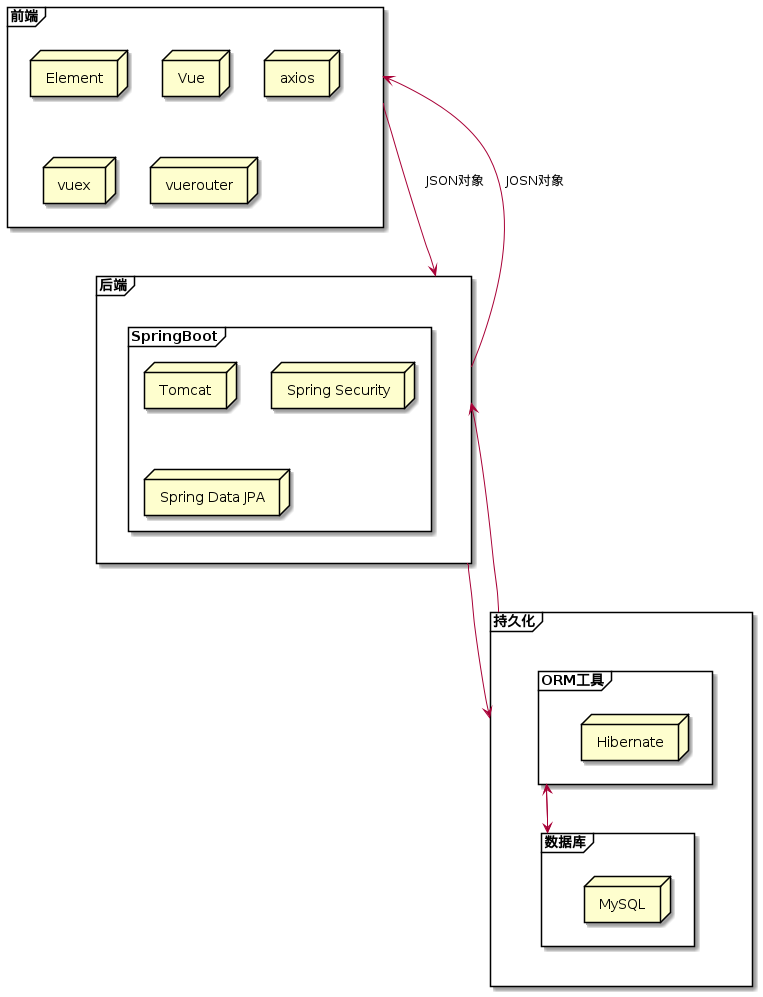
\includegraphics[scale = 0.46]{out/uml/部署图/系统架构/系统架构.png}
    \caption{\song\wuhao 系统架构设计}
    \label{system-frame-deployment}
\end{figure}

\section{系统整体模块设计}

系统整体模块设计如图\ref{system-wbs}所示,总体可以分为学生模块,教师模块,管理员模块。在学生模块中可以进一步将功能细分为论文上传功能,论文下载功能,成绩查看功能,回复评论功能,论文更新功能。教师模块可以进一步分为查看所管理的学生论文信息功能,论文下载功能,论文评论功能,论文添加问题标签功能,论文评分功能。管理模块可以进一步分为系统管理和论文管理,系统管理可以进一步分为用户管理,上传通道管理,论文管理可以进一步分为评审情况统计,教师评审情况统计。

\begin{figure}[htbp]
    \centering
    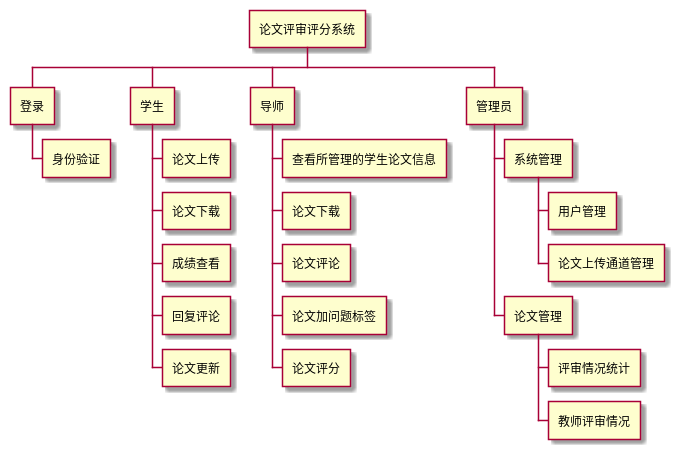
\includegraphics[scale = 0.6]{out/uml/WBS/系统WBS/系统WBS.png}
    \caption{\song\wuhao 系统整体模块}
    \label{system-wbs}
\end{figure}

\subsection{文件上传模块}

\begin{figure}[htbp]
    \centering
    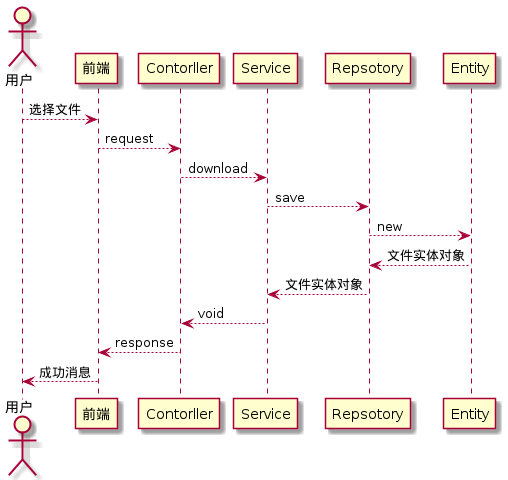
\includegraphics[scale = 0.6]{out/uml/时序图/file-upload-sequence/file-upload-sequence.png}
    \caption{\song\wuhao 文件上传时序图}
    \label{file-upload-sequence}
\end{figure}

如图\ref{file-upload-sequence}所示,首先用户点击上传文件按钮,选择文件后前端会发起上传请求,请求体中会包含二进制文件以及文件信息,Controller接收到请求之后,从请求体中取出文件,并获取文件名,文件类型,文件数据,通过Spring Security 的机制可以获取到用户信息,这样一个文件实体所需要的所有信息都可以获得(文件名,文件类型,文件数据,文件所属学生id),将创建的文件实体传递给Service,Service调用文件Repository将文件实体持久化。该流程完毕之后,数据库文件表会增加一条数据。

\subsection{文件下载模块}

\begin{figure}[htbp]
    \centering
    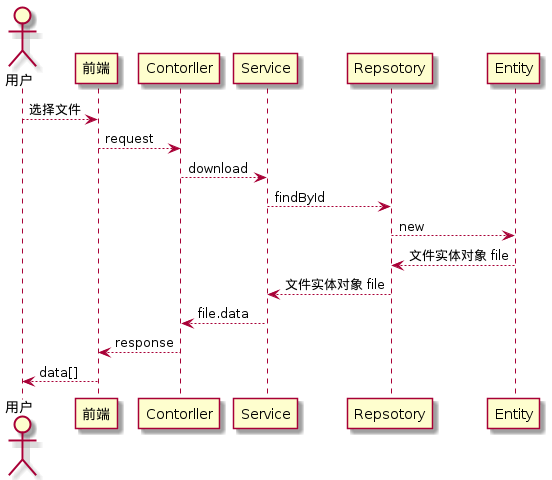
\includegraphics[scale = 0.6]{out/uml/时序图/file-download-sequence/file-download-sequence.png}
    \caption{\song\wuhao 文件下载时序图}
    \label{file-download-sequence}
\end{figure}

如图\ref{file-download-sequence}所示,首先用点击文件下载按钮,之后前端会发起下载请求,url参数会有想要下载的文件id,Controller接收到请求之后,解析出需要获取的文件id,将id传递给Service,Service使用文件Repository通过id查询数据库,并利用查询到的数据生成文件实体,将实体中的data[]即二进制文件数据返还给Controller,Controller将response返还给前端,前端解析出文件并下载。

\subsection{文件更新模块}

\begin{figure}[htbp]
    \centering
    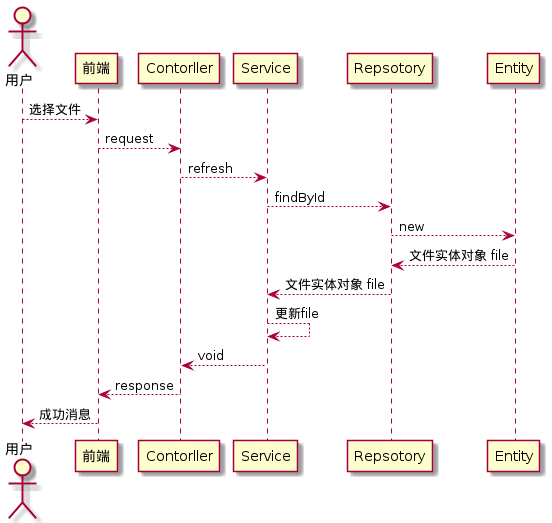
\includegraphics[scale = 0.6]{out/uml/时序图/file-refresh-sequence/file-refresh-sequence.png}
    \caption{\song\wuhao 文件更新时序图}
    \label{file-refresh-sequence}
\end{figure}

如图\ref{file-refresh-sequence}所示,首先用户点击文件更新按钮,之后前端会发起更新文件请求,请求体中会带有新的二进制文件以及要更新的文件id,Controller接收到请求之后,解析出文件和文件id,将两者传递给Service,Service首先会重数据库中取出原来的文件,然后使用新传来的文件信息更新旧文件,最后再将更新后的文件使用文件Repository写回数据库。之后Controller返回表示成功的response给前端。

\subsection{文件评论模块}

学生和教师都可以针对一个文件进行评论,用户双方的沟通,教师可以使用评论功能提出文章的问题,学生可以根据教师的回复进行对文章的更改,更改之后更新文章。如图\ref{file-comment-sequence}所示,用户首先选择要评论的文件并填入评论内容,前端发起请求,请求体中带有文件id,父级评论id和评论内容,Controller接收到请求之后,将二者转交给Service处理,Service需要创建一个评论实体,需要填入评论内容,为哪个文件评论(文件id),由谁评论(从principal中可以取出发送请求的用户信息),回复哪一条评论(父级评论id),这些信息便可以确定唯一一条评论,之后使用CommentRepository保存,将信息持久化。

\begin{figure}[htbp]
    \centering
    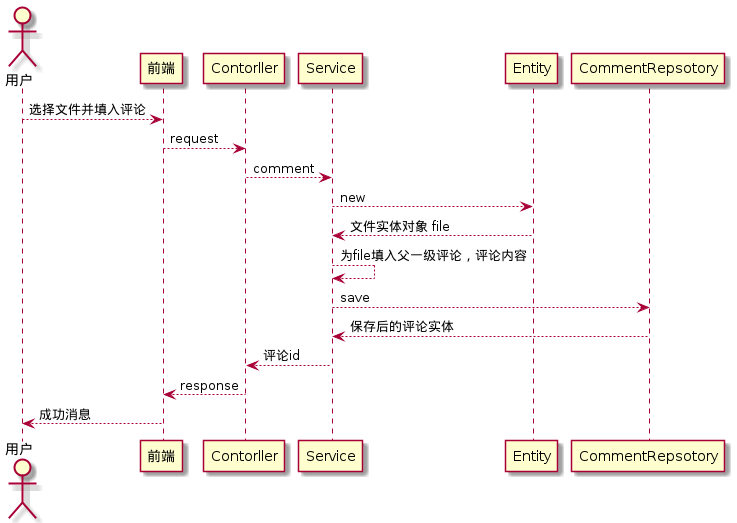
\includegraphics[scale = 0.6]{out/uml/时序图/file-comment-sequence/file-comment-sequence.png}
    \caption{\song\wuhao 文件评论时序图}
    \label{file-comment-sequence}
\end{figure}

\subsection{问题标签模块}

\begin{figure}[htbp]
    \centering
    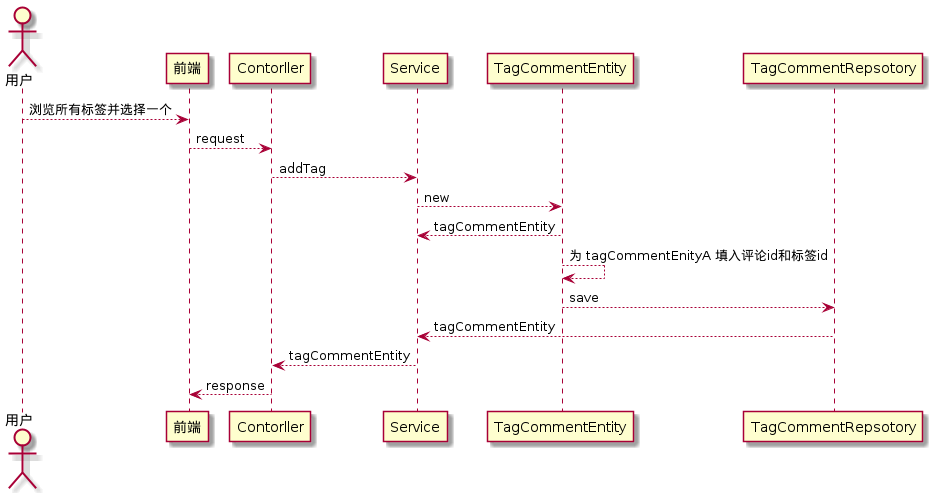
\includegraphics[scale = 0.45]{out/uml/时序图/file-tag-sequence/file-tag-sequence.png}
    \caption{\song\wuhao 问题标签时序图}
    \label{file-tag-sequence}
\end{figure}

在教师为文章评论时,教师可以为同时为评论添加问题标签,便于学生快速了解到文章的问题所在,标签也可以用于后序的论文问题统计。如图\ref{file-tag-sequence}所示,用户可以在评论上点击添加问题标签,当选择标签并且确定之后前端将发起一个请求,Controller接收到请求之后,从请求体中解析出评论id和所有的标签id并将其传递给Service进行处理,Service新建一个TagComment对象,填充评论属性和标签属性并使用Repository将数据保存到数据库。

\subsection{论文评分模块}

\begin{figure}[htbp]
    \centering
    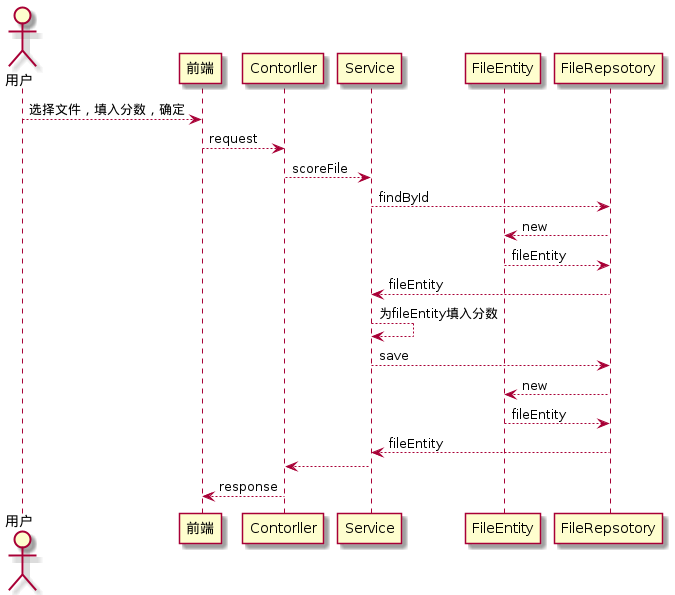
\includegraphics[scale = 0.6]{out/uml/时序图/file-score-sequence/file-score-sequence.png}
    \caption{\song\wuhao 论文评分时序图}
    \label{file-score-sequence}
\end{figure}

当教师认为论文达到评审标准之后可以对论文进行评分。如图\ref{file-score-sequence}所示,教师点击评分按钮弹出对话框,可以滑动对话框中的滑动条进行分数选择,点击确定按钮,前端将发起评分请求,Controller接收到请求之后,可以解析出文件的id和分数,Controller将两个参数传递给Service,Service调用Repository根据文件id查询数据库返回文件实体对象,Service操作实体对象填入分数并调用Repository的方法将数据保存回数据库。

\subsection{论文得分情况统计模块}

\begin{figure}[htbp]
    \centering
    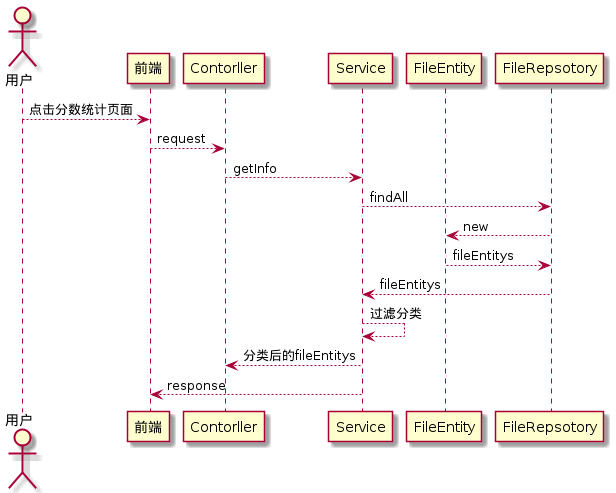
\includegraphics[scale = 0.6]{out/uml/时序图/statistic-score-sequence/statistic-score-sequence.png}
    \caption{\song\wuhao 统计分数时序图}
    \label{statistic-score-sequence}
\end{figure}

如图\ref{statistic-score-sequence}所示,管理员点击得分总览页面,前端向后台发起请求,Controller接到请求之后请求Service服务,Service从数据库取出所有论文信息并总动填充为文件实体的list,之后根据文件的得分情况进行分类,分类后的数据从Service传回Controller,之后Controller将返回输入放入response返还给前端,前端使用Echarts可视化展示给用户。

\subsection{教师任务完成请求统计模块}

\begin{figure}[htbp]
    \centering
    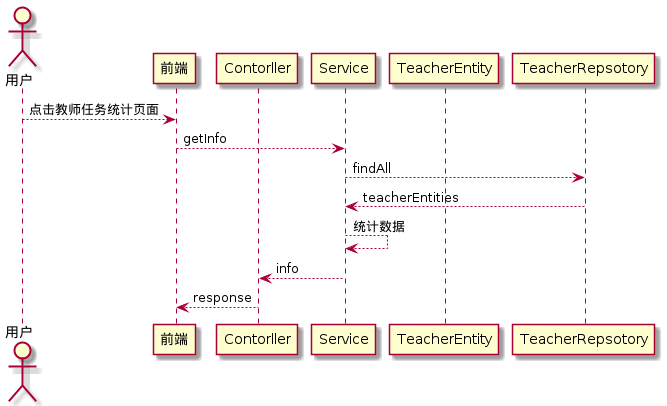
\includegraphics[scale = 0.6]{out/uml/时序图/statistic-teacher-task-sequence/statistic-teacher-task-sequence.png}
    \caption{\song\wuhao 统计教师任务完成情况时序图}
    \label{statistic-teacher-task-sequence}
\end{figure}

如图\ref{statistic-teacher-task-sequence}所示,管理员点击学生任务统计页面,前端向后台发起请求,Controller接到请求Service服务,Service从数据库取出所有的教师信息,其中与教师关联的学生属性会由Hibernate框架填充,同样的,学生的论文属性也会被填充,这样就可以获得所有与教师任务相关的信息,也就可以进行分离,Service将分类后的数据返还给Controller,Controller将其放入response中发还给前端,前端使用Echarts进行可视化处理展示给用户。

\subsection{学生管理模块}

\begin{figure}
    \centering
    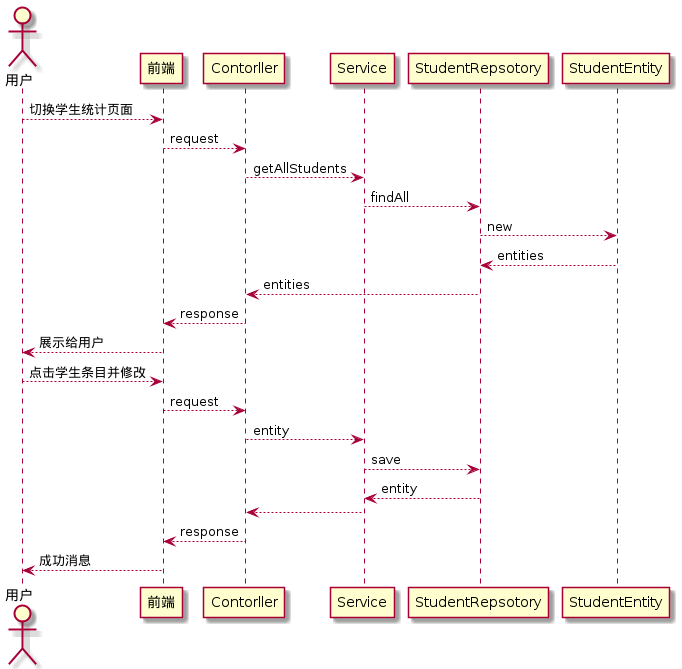
\includegraphics[scale = 0.6]{out/uml/时序图/manage-student-sequence/manage-student-sequence.png}
    \caption{\song\wuhao 学生管理时序图}
    \label{manage-student-sequence}
\end{figure}

如图\ref{manage-student-sequence}所示,当管理员切换到学生管理页面,前端向后端发起请求,Controller接收到请求之后调用Service,Service使用Repository查询出所有的学生信息并映射为学生实体,之后返还给Controller,Controller将其附加在response返还给前端进行展示。用户可以点击学生条目,进行修改,修改后点击确认,前端将向后端发起请求,Controller接收到请求之后可以解析出学生实体,Controller调用Service,Service将调用Repository将实体保存(因为该实体id属性不为空,所以会更新id相同的那一条学生信息)。

\subsection{教师管理模块}

\begin{figure}
    \centering
    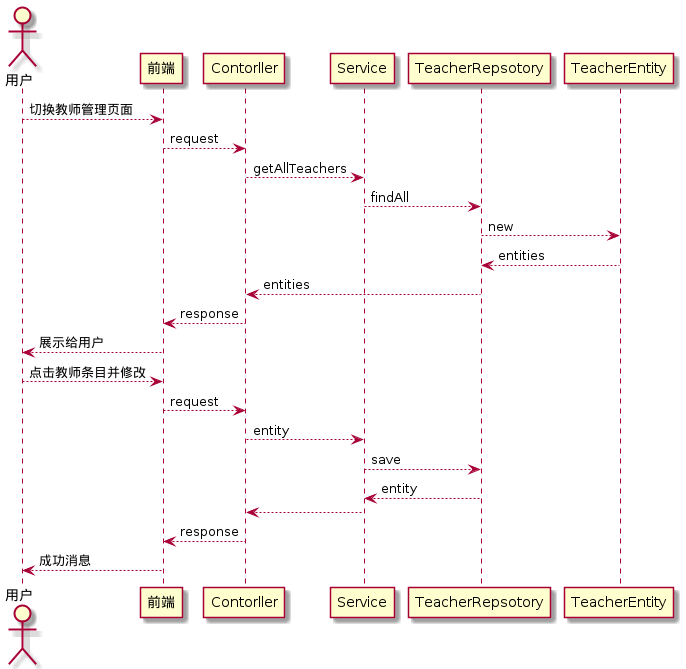
\includegraphics[scale = 0.6]{out/uml/时序图/manage-teacher-sequence/manage-teacher-sequence.png}
    \caption{\song\wuhao 教师管理时序图}
    \label{manage-teacher-sequence}
\end{figure}

如图\ref{manage-teacher-sequence}所示,当管理员切换到学生管理页面,前端向后端发起请求,Controller收到请求之后使用Service获取所有教师信息,其中Service会调用Repository查询数据库并将教师信息映射为实体对象,Controller将获得的所有教师信息放入response中返还给前端,用户可以点击教师条目,在对话框中修改教师信息,点击确认之后前端将发起修改请求,Controller接收到请求之后可以从请求中解析出教师实体,之后使用Repository使用这个新的教师实体对象更新旧的教师数据。

\section{数据库设计}

在数据库设计的过程中除了需要考虑范式的问题,也需要考虑系统所选用的ORM框架的特点,Hibernate不同于半自动的MyBatis框架,作为一个全自动的框架,它对于表设计的要求更高,因为面向对象编程(OOPs)基于实体,而关系数据库管理系统(RDBMS)依赖关系和字段来存储数据\cite{Dhingra2017ReviewOJ},在设计过程中需要在两者之间做出权衡。Hibernate用户必须实现特定的方法和注释特定的类,以正确地存储和检索数据库中的元素。如果应用程序的代码没有遵循这些建议,在极端情况下,不符合体系结构规则甚至可能导致数据丢失\cite{10.1145/3350768.3351796}。

\subsection{概念结构设计}

\begin{figure}[htbp]
    \centering
    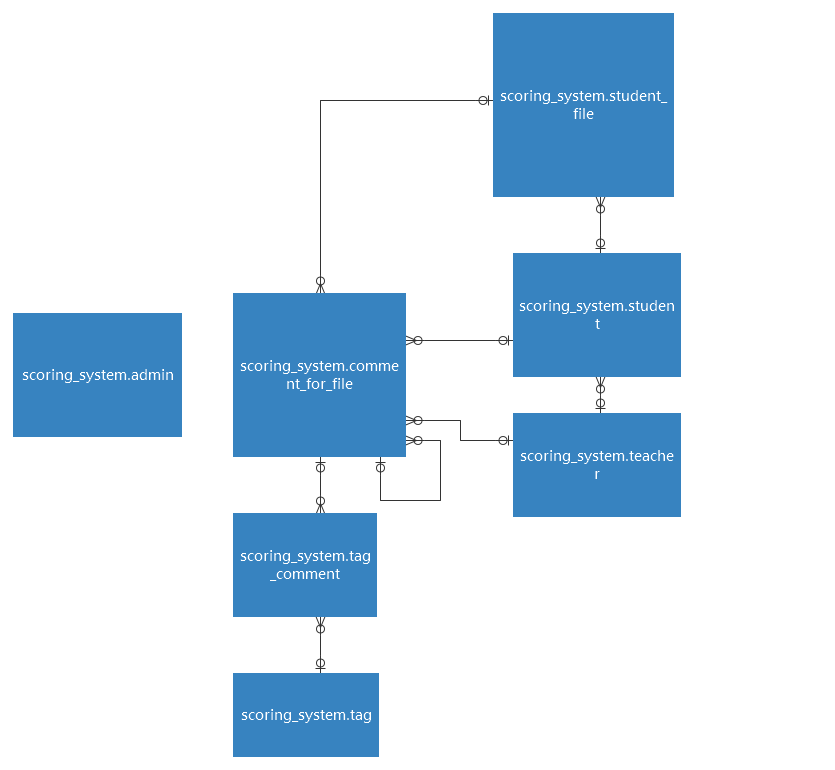
\includegraphics[scale = 0.5]{out/uml/数据库/conceptual-model.png}
    \caption{\song\wuhao 概念模型}
    \label{conceptual-model}
\end{figure}

如图\ref{conceptual-model}所示,本系统一共有三种用户,学生(student)、教师(teacher)以及管理员(admin),每一个教师拥有多个学生,每个学生分给一个教师。每一名学生拥有多篇论文(student\_file),每一篇论文可以有多个评论(comment\_for\_file),每条评论可以添加多个问题标签(tag),同一个标签可以被多条论文引用,所以标签和评论之间是多对多的关系,因此需要一个连接表(tag\_comment)。

\subsection{逻辑结构设计}

如图\ref{logical-model}所示,

(1) 学生表

id作为学生序号,该字段自增且为主键,不能为空。name字段为学号,根据学校要求进行编码,又有学号可能有字母例如“student0001”等等用于学生类型分类,所以该字段选择使用String类型,password字段为学生密码,由于密码可以使用字母和数字,所以这里选择String类型,teacher\_id字段表示该学生分配给哪一名教师管理,由于教师id字段为Integer类型,所以teacher\_id字段也为Integer类型。

(2) 教师表

共有三个字段,id,name和password,详细介绍类似学生表三个同名字段。

(3) 管理员表

共有三个字段,id,name和password,详细介绍类似学生表三个同名字段。

(4) 论文表

id字段作为论文编号,该字段自增且为主键,不能为空,选择Integer类型;data字段为 byte[] 类型,用于存放二进制文件数据;name字段为文件名,为String类型;score字段存放论文得分,选择Integer类型;type字段用于存放文件类型,例如pdf,word,选择String类型;student\_id字段指示该论文属于哪一名学生,因此该字段为外键,引用学生表的id字段;file\_abstract字段为论文摘要,使用String类型。

(5) 评论表

id字段作为评论编号,该字段自增且为主键,不能为空,选择Integer类型;comments字段为评论的具体内容,选择String类型;parent\_comemnt\_id字段指示该条评论是回复哪一条评论的,该字段为外键应用评论表的id字段,所以为Integer类型;student\_file\_id字段指示该评论是在那一篇论文下回复的,该字段为外键,引用论文表的id字段,因此为Integer类型;student\_id字段指示该条评论是哪一名学生回复的,该字段为外键,引用学生表的id字段,因此为Integer类型,如果这条评论是教师回复的,那么该字段的值为null;teacher\_id字段指示该条评论是哪一名教师回复的,该字段为外键,引用教师表的id字段,因此为Integer类型,如果这条评论是学生回复的,那么该字段的值为null。

(6) 标签表

id字段作为标签编号,该字段自增且为主键,不能为空,选择Integer类型;name字段为标签名字,使用String类型。

(7) 评论标签表

该表用于记录某一条评论引用了哪一个标签,为多对多。id字段作为引用记录的id,该字段自增且为主键,不能为空,使用Integer类型;comment\_id指示为哪一条评论添加标签,该字段为外键,引用评论表的主键id字段;tag\_id字段指示为这条评论添加哪一个标签,该字段为外键,引用标签表的主键id字段。

\begin{figure}[htbp]
    \centering
    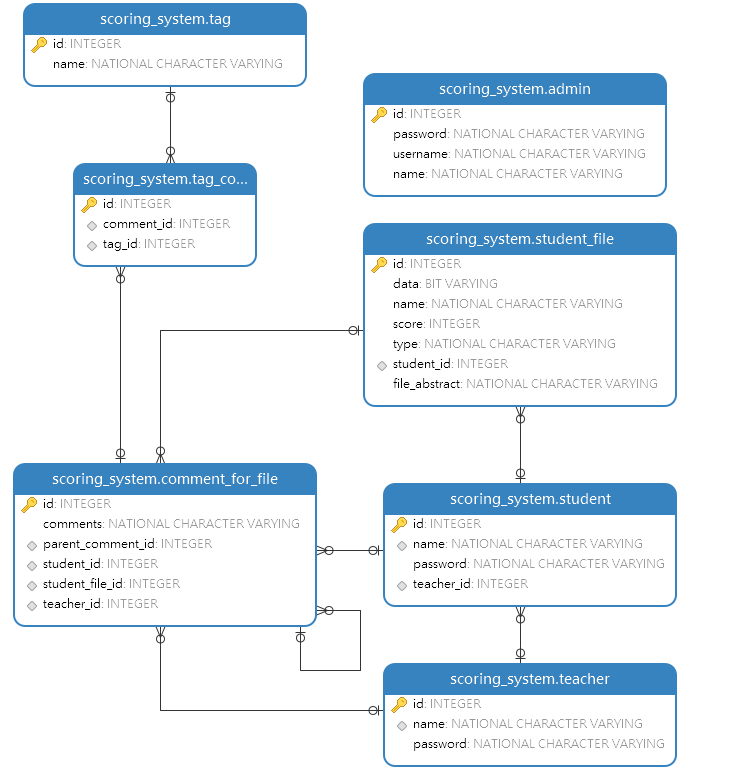
\includegraphics[scale = 0.5]{out/uml/数据库/logical-model.png}
    \caption{\song\wuhao 逻辑模型}
    \label{logical-model}
\end{figure}

\subsection{物理结构设计}

如图\ref{physical-model}所示,

\begin{figure}[htbp]
    \centering
    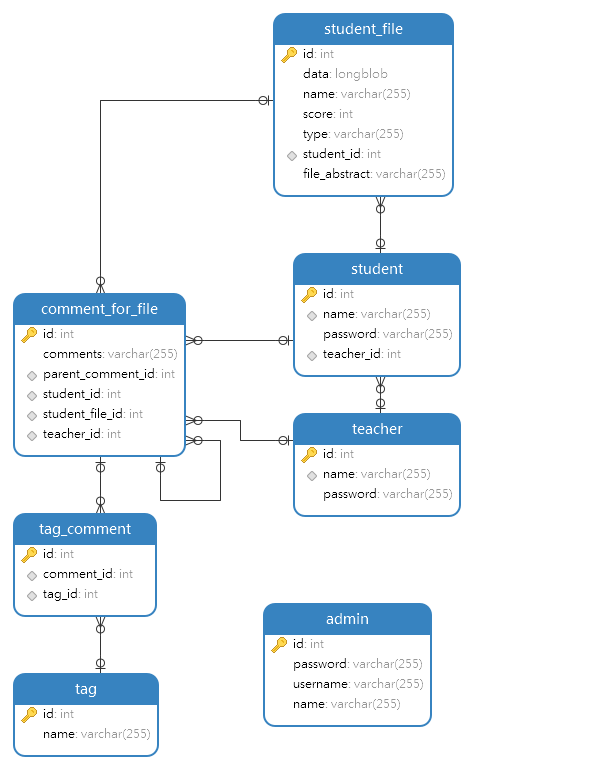
\includegraphics[scale = 0.6]{out/uml/数据库/physical-model.png}
    \caption{\song\wuhao 物理模型}
    \label{physical-model}
\end{figure}

(1)  学生表

如图\ref{db-student}所示,学生表id字段使用int类型;学生表name(编号)字段使用varchar(255)类型;学生表password(密码)字段使用varchar(255)类型;学生表teacher\_id(所属教师id)字段使用int类型;
\begin{table}[]
    \centering
    \song\wuhao
    \caption{学生表}
    \label{db-student}
    \begin{tabular}{lllllll}
        \hline
        列名        & 数据类型     & 字段类型 & 长度 & 是否为空 & 默认值 & 备注     \\ \hline
        id          & int          & int      & null & NO       & null   & 学生id   \\
        name        & varchar(255) & varchar  & 255  & YES      & null   & 学生姓名 \\
        password    & varchar(255) & varchar  & 255  & YES      & null   & 学生密码 \\
        teacher\_id & int          & int      & null & YES      & null   & 教师id   \\ \hline
    \end{tabular}
\end{table}

(2)  教师表

如图\ref{db-teacher}所示,共有三个字段,id,name和password,详细介绍类似学生表三个同名字段。
\begin{table}[htbp]
    \centering
    \song\wuhao
    \caption{教师表}
    \label{db-teacher}
    \begin{tabular}{lllllll}
        \hline
        列名     & 数据类型     & 字段类型 & 长度 & 是否为空 & 默认值 & 备注     \\ \hline
        id       & int          & int      & null & NO       & null   & 教师id   \\
        name     & varchar(255) & varchar  & 255  & YES      & null   & 教师编号 \\
        password & varchar(255) & varchar  & 255  & YES      & null   & 教师密码 \\ \hline
    \end{tabular}
\end{table}

(3)  管理员表

如图\ref{db-admin}所示,共有三个字段,id,name和password,详细介绍类似学生表三个同名字段。
\begin{table}[htbp]
    \centering
    \song\wuhao
    \caption{管理员表}
    \label{db-admin}
    \begin{tabular}{lllllll}
        \hline
        列名     & 数据类型     & 字段类型 & 长度 & 是否为空 & 默认值 & 备注       \\ \hline
        id       & int          & int      & null & NO       & null   & 管理员id   \\
        name     & varchar(255) & varchar  & 255  & YES      & null   & 管理员名称 \\
        password & varchar(255) & varchar  & 255  & YES      & null   & 管理员密码 \\ \hline
    \end{tabular}
\end{table}

(4)  论文表

如图\ref{db-file}所示,论文表id(论文编号)字段使用int类型;论文表data(论文二进制数据)字段使用longblob类型;论文表name(论文题目)字段使用varchar(255)类型;论文表score(论文得分)字段使用int类型;论文表type(论文文件的类型)字段使用varchar(255)类型;论文表student\_id(论文所属学生编号)字段使用int类型;论文表file\_abstract(论文摘要内容)字段使用varchar(255)类型。
\begin{table}[htbp]
    \centering
    \song\wuhao
    \caption{论文表}
    \label{db-file}
    \begin{tabular}{lllllll}
        \hline
        列名           & 数据类型     & 字段类型 & 长度     & 是否为空 & 默认值 & 备注             \\ \hline
        data           & longblob     & longblob & 4.29E+09 & YES      & null   & 文章数据         \\
        file\_abstract & varchar(255) & varchar  & 255      & YES      & null   & 文章摘要         \\
        id             & int          & int      & null     & NO       & null   & 文章id           \\
        name           & varchar(255) & varchar  & 255      & YES      & null   & 文章名           \\
        score          & int          & int      & null     & YES      & null   & 文章得分         \\
        student\_id    & int          & int      & null     & YES      & null   & 文章所属的学生id \\
        type           & varchar(255) & varchar  & 255      & YES      & null   & 文件类型         \\ \hline
    \end{tabular}
\end{table}

(5)  评论表

如图\ref{db-comment}所示,评论表id(评论编号)字段使用int类型;评论表comments(评论内容字段)使用varchar(255)类型;评论表parent\_comment\_id(指明该评论是回复哪一条评论的)使用int类型;评论表student\_id(指明是哪一名学生写的此条评论)使用int类型;评论表teacher\_id(指明这条评论是哪一名教师写的)使用int类型;评论表student\_file\_id(指明该条评论是回复哪一条论文的)。
\begin{table}[htbp]
    \centering
    \song\wuhao
    \caption{评论表}
    \label{db-comment}
    \begin{tabular}{lllllll}
        \hline
        列名                & 数据类型     & 字段类型 & 长度 & 是否为空 & 默认值 & 备注     \\ \hline
        comments            & varchar(255) & varchar  & 255  & YES      & null   & 评论内容 \\
        id                  & int          & int      & null & NO       & null   & 评论id   \\
        parent\_comment\_id & int          & int      & null & YES      & null   & 父级评论 \\
        student\_file\_id   & int          & int      & null & YES      & null   & 论文id   \\
        student\_id         & int          & int      & null & YES      & null   & 学生id   \\
        teacher\_id         & int          & int      & null & YES      & null   & 教师id   \\ \hline
    \end{tabular}
\end{table}

(6)  标签表

如图\ref{db-tag}所示,标签表id(标签编号)字段使用int类型;标签表name(标签名字)字段使用varchar(255)类型。
\begin{table}[htbp]
    \centering
    \song\wuhao
    \caption{标签表}
    \label{db-tag}
    \begin{tabular}{lllllll}
        \hline
        列名 & 数据类型     & 字段类型 & 长度 & 是否为空 & 默认值 & 备注       \\ \hline
        id   & int          & int      & null & NO       & null   & 问题标签id \\
        name & varchar(255) & varchar  & 255  & YES      & null   & 问题标签名 \\ \hline
    \end{tabular}
\end{table}

(7)  评论标签表

如图\ref{db-tag-comment}所示,评论标签表id(添加标签记录编号)字段使用int类型;标签评论表comment\_id(指明将标签添加到哪一条评论上)使用int类型;标签评论表tag\_id(指明将哪一个tag添加到评论上)使用int类型。
\begin{table}[]
    \centering
    \song\wuhao
    \caption{标签评论表}
    \label{db-tag-comment}
    \begin{tabular}{lllllll}
        \hline
        列名        & 数据类型 & 字段类型 & 长度 & 是否为空 & 默认值 & 备注               \\ \hline
        comment\_id & int      & int      & null & YES      & null   & 所属评论id         \\
        id          & int      & int      & null & NO       & null   & tag使用记录id      \\
        tag\_id     & int      & int      & null & YES      & null   & 使用的问题标签的id \\ \hline
    \end{tabular}
\end{table}

\section{本章小结}

本章的主要内容是系统设计,首先对系统的整体架构进行了简单介绍并且谈论了选择该架构的原因,其次介绍了系统各个模块的功能以及工作流程,然后详细介绍了论文评审评分系统的数据库设计。
